\documentclass[UTF8]{article}

\usepackage{ctex}
\usepackage{amsmath}
\usepackage{bm}
\usepackage{amsfonts}
\usepackage{graphicx}
\usepackage{subfigure}

\begin{document}
\quad\\
勘误修订\quad\\ \quad
[本书因颇受欢迎,出版社提出重印,于是作者借机要求在每次重印时加入新的修订,省却让读者等待第二版的麻烦。为方便读者,所有修订内容都列举在此。其中部分修订是为了更便于读者理解,并非原文有误]

\quad\\
(第一版第30次印刷, 2018年12月):
\\
p.38, 式(2.27):"$\max$" --> "$\min$" \\
p.39, 倒数第1行: "若平均错误率……临界值范围"  --> "若~$\tau_t$~位于临界值范围" \\
p.152, 第10行: "6/8 = 0.750" --> "5/8 = 0.625" \\
p.153, 第3行: "0.063" --> "0.052" \\
p.153, 第6行: "0.063" --> "0.052" \\
p.172, 式(8.2): "$H$" --> "$F$" \\
p.173, 式(8.3): "$H$" --> "$F$" \\
p.174, 图8.3最后一行: "$H$" --> "$F$" \\
p.175, 式(8.12)前一行: "最小化" --> "最小化~$\ell_{\rm exp}(H_{t-1} + \alpha_t h_t \mid \mathcal{D})$, 可简化为最小化" \\
p.185, 式(8.28)前一行: "是" --> "定义为" \\
p.284, 倒数第三行:"$y_i =$" --> "$y_i \in$"
\\
\\
(第一版第29次印刷, 2018年11月)
\\
(第一版第28次印刷, 2018年8月)
\\
(第一版第27次印刷, 2018年6月):
\\
p.42, 表2.5后第四行:"$(k^2-1)/12$" --> "$(k^2-1)/12N$" \\
p.159, 倒数第9行、第10行中两处: "字节长度" --> "编码位数" \\
p.160, 第1行、第4行中两处: "字节数" --> "编码位数" \\
p.160, 第7行、第10行中两处: "字节" --> "编码位" \\
p.174, 式(8.7)中两处、(8.8)中 7 处、边注中两处: "$f(x)$" --> "$f(\bm{x})$" \\
\\
(第一版第26次印刷, 2018年5月):
\\
p.58, 倒数第二行:"对率函数" --> "下面我们会看到, 对率回归求解的目标函数" \\
p.230, 倒数第三行:"方差" --> "协方差矩阵" \\
\\
(第一版第25次印刷, 2018年3月):
\\
p.39, 最后一行:"$[-\infty,$" --> "$(-\infty,$","$, \infty]$" --> "$, \infty)$" \\
p.199, 式(9.12):分母的 "$(\bm{\mu}_i, \bm{\mu}_j)$" --> "$(C_i, C_j)$" \\
\\
(第一版第24次印刷, 2018年1月):
\\
p.112, 图 5.14a: 修订文件 参考Fig5.14a.pdf \\
p.303, 倒数第二行:去掉 "[Zhou et al., 2004]" \\
p.304, 第一行:"当" --> "考虑到有标记样本通常很少而未标记样本很多, 为缓解过拟合, 可在式(13.21)中引入针对未标记样本的~L$_2$~范数项~$\mu \sum_{i=l+1}^{l+u}\|\mathbf{F}_{i}\|^{2}$, 在"; 同时插入边注: "参见~11.4~节" \\
\\
(第一版第23次印刷, 2017年10月):
\\
p.27, 式(2.1):第一个"$\mapsto$" --> "$\to$", 第二个"$\mapsto$" --> "$=$" \\
p.80, 倒数第2行:"算法4.2" --> "图 4.2 算法" \\
p.131, 图 6.5: 修订文件 参考mlbookfig65.pdf\\
\\
(第一版第22次印刷, 2017年9月):
\\
p.156, 倒数第7行:"(7.23)" --> "(7.21)" \\
p.320, 第8行:"其余~$n-2$" --> "此前~$t-2$" \\
\\
(第一版第21次印刷, 2017年8月)
\\
(第一版第20次印刷, 2017年7月):
\\
p.60, 图3.3中:"$y = \bm{w}^{\rm T}\bm{x}$, $y$" --> "投影方向~$\bm{w}$" \\
p.133, 式(6.42)加边注: "传统意义上的"结构风险"是指引入模型结构因素后的总体风险(或许更宜译为"带结构风险"), 本书则是指总体风险中直接对应于模型结构因素的部分, 这样从字面上更直观, 或有助于理解其与机器学习中其他内容间的联系. 参见p.160." \\
\\
(第一版第19次印刷, 2017年6月):
\\
p.159, 第一行加边注:"一般需先对图剪枝, 仅保留有向图中~$x$, $y$, $\bf{z}$~及它们的祖先结点" \\
p.230, 式(10.15)上面一行加边注: "严格来说, 协方差矩阵是~${1 \over {m-1}}\sum\nolimits_{i=1}^m\bm{x}_i\bm{x}_i^{\rm T}$, 但前面的常数项在此不发生影响"
\\
(第一版第18次印刷, 2017年5月):
\\
p.187, 式(8.39)下面一行: "$\le$" --> "$\ge$" \\
\\
(第一版第17次印刷, 2017年4月):
\\
p.384, 图16.10, 步骤9: "$\pi(x, a)$" --> "$\pi(x)$" \\
p.388, 图16.13, 步骤4: "$\pi^{\epsilon}(x)$" --> "$a = \pi^{\epsilon}(x)$" \\
p.388, 图16.13, 步骤8: 去掉", $a = a'$" \\
\\
(第一版第16次印刷, 2017年3月):
\\
p.417, 第3段第1行: "通往人工智能的途径" --> "一种人工智能途径" \\
\\
(第一版第15次印刷, 2017年2月):
\\
p.206, 9.4.3节前倒数第5行: "$c_2$" --> "$c_1$" \\
\\
(第一版第14次印刷, 2016年12月):
\\
p.34, 图 2.4(b): 修订文件\\
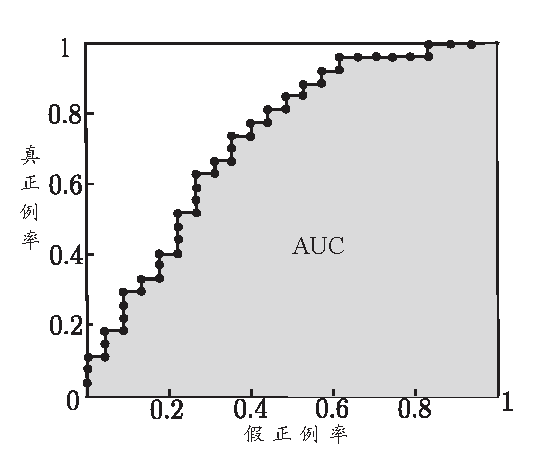
\includegraphics{pic/mlbookfig24b.eps} \\
p.206, 9.4.3节前倒数第2行: "(0.722; 0.442)" --> "(0.722; 0.447)" \\
p.209, 式(9.38)上面一行: "样本" --> "混合成分" \\
p.215, 图9.11第5步: "$j = 1, 2, \ldots, m$" --> "$j = i+1, \ldots, m$" \\
p.230, 式(10.14)结尾: "." --> "," \\
p.230, 式(10.14)下面一行开头顶格插入: "其中${\bf W} = (\bm{w}_1, \bm{w}_2, \ldots, \bm{w}_d)$." \\
p.231, 式(10.17): 两处"${\bf W}$"-->"${\bm w}_i$", "$\lambda$" --> "$\lambda_i$" \\
p.231, 式(10.17)下面第二行: "${\bf W}$" --> "${\bf W}^*$" \\
p.231, 图10.5最后一行: "${\bf W}$" --> "${\bf W}^*$" \\
p.232, 第一行: "${\bf W}$" --> "${\bf W}^*$" \\
p.232, 式(10.19)前第二行: "${\bf W}$" --> "${\bf W} = (\bm{w}_1, \bm{w}_2, \ldots, \bm{w}_d)$" \\
p.232, 式(10.19)前第二行: "即PCA欲求解" --> "则对于 $\bm{w}_j$, 由式(10.17)有" \\
p.232, 式(10.19): 两处"${\bf W}$"-->"${\bm w}_j$"; "$\lambda$" --> "$\lambda_j$" \\
p.233, 式(10.20): 三处"${\bf W}$"-->"${\bm w}_j$"; 两处"$\lambda$"-->"$\lambda_j$"; "${\bm \alpha}_i$"-->"$\alpha_i^j$" \\
p.233, 式(10.20)下一行: "${\bm \alpha}_i$"-->"$\alpha_i^j$"; "$\lambda$"-->"$\lambda_j$"; "${\bf W}$"-->"${\bm w}_j$" \\
p.233, 式(10.20)下一行: ". 假定" --> "是${\bm \alpha}_i$的第$j$个分量. 假定" \\
p.233, 式(10.21): 两处"${\bf W}$"-->"${\bm w}_j$"; "$\lambda$"-->"$\lambda_j$" \\
p.233, 式(10.22): "${\bf W}$"-->"${\bm w}_j$"; "${\bm \alpha}_i$"-->"$\alpha_i^j$" \\
p.233, 式(10.24): 两处"${\bf A}$"-->"${\bm \alpha}^j$"; "$\lambda$"-->"$\lambda_j$" \\
p.233, 式(10.24)下面一行: "${\bf A} = ({\bm \alpha}_1; {\bm \alpha}_2; \ldots; {\bm \alpha}_m)$" --> "${\bm \alpha}^j = (\alpha_1^j; \alpha_2^j; \ldots; \alpha_m^j)$" \\
p.233, 式(10.25)下面一行: 去掉 ", $\alpha_i^j$ 是 ${\bm \alpha}_i$ 的第 $j$ 个分量" \\
\\
(第一版第13次印刷, 2016年11月):
\\
p.36, 倒数第5行: "(TPR, FPR)" --> "(FPR, TPR)" \\
p.120, 第7行: "(1927 -- )" --> "(1927 -- 2016)" \\
p.203, 图9.2下面一行: "$\bm{x}_{27}$" --> "$\bm{x}_{24}$" \\
p.203, 图9.2下面第3行: "(0.532; 0.472)" --> "(0.478; 0.437)" \\
p.203, 图9.2下面第5行: "0.166" --> "0.220" \\
p.203, 图9.2下面第7行: 大括号中增加 "$\bm{x}_3$", 去掉"$\bm{x}_{15}$" \\
p.203, 倒数第5行: 大括号中去掉 "$\bm{x}_3$", 增加"$\bm{x}_{15}$" \\
p.203, 倒数第3行: "(0.473; 0.214)" --> "(0.493; 0.207)" \\
p.203, 倒数第3行: "(0.623; 0.388)" --> "(0.602; 0.396)" \\
p.204, 图9.3: 修订文件     \\
\begin{figure}
	\centering
	\subfigure[9.3a]{
		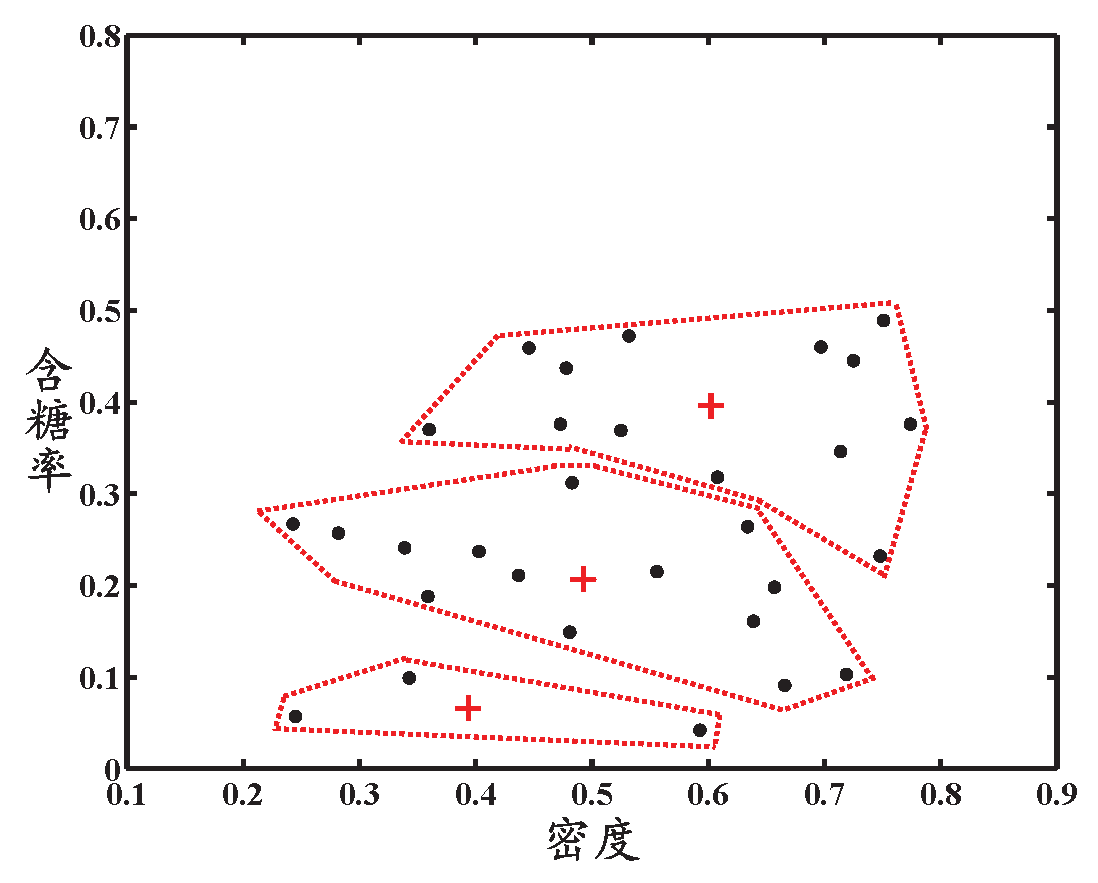
\includegraphics[width=0.45\textwidth]{pic/Fig9.3a.eps} 
	}
	\subfigure[9.3b]{
		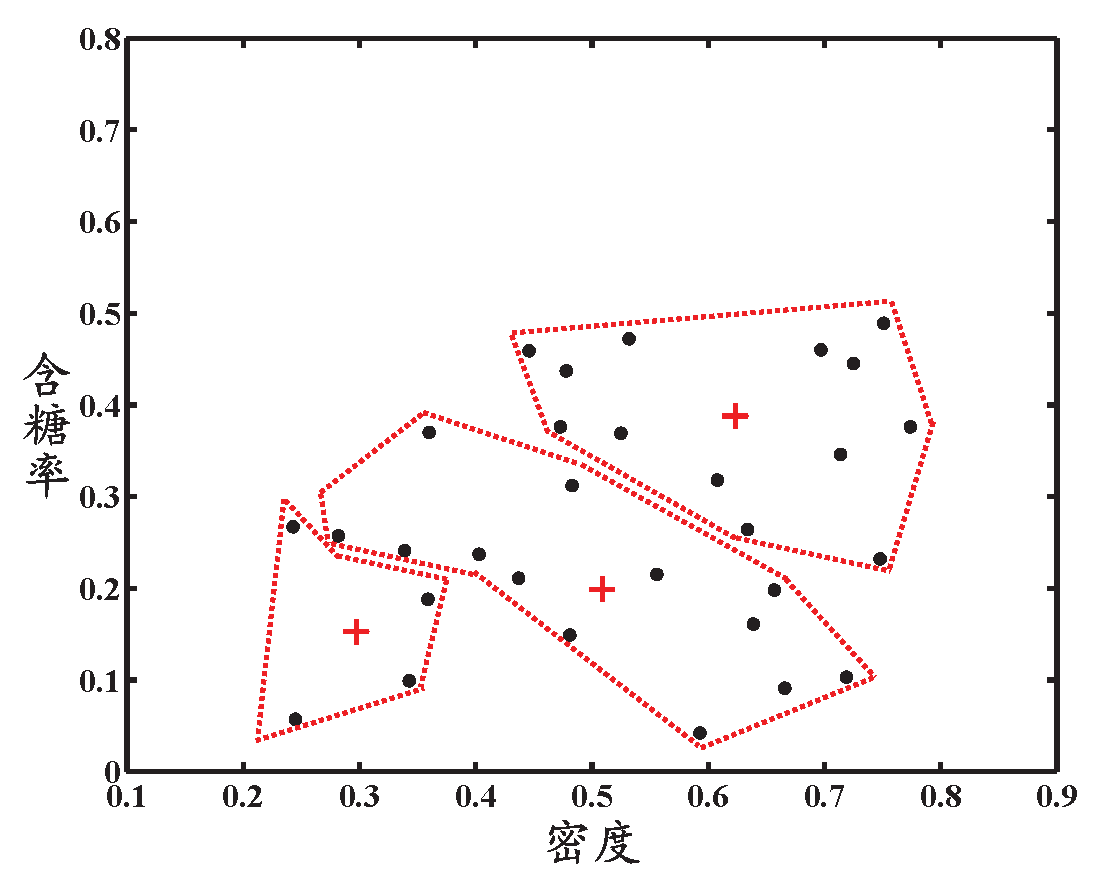
\includegraphics[width=0.45\textwidth]{pic/Fig9.3b.eps}
	}
\end{figure}
\begin{figure}
	\centering
	\subfigure[9.3c]{
		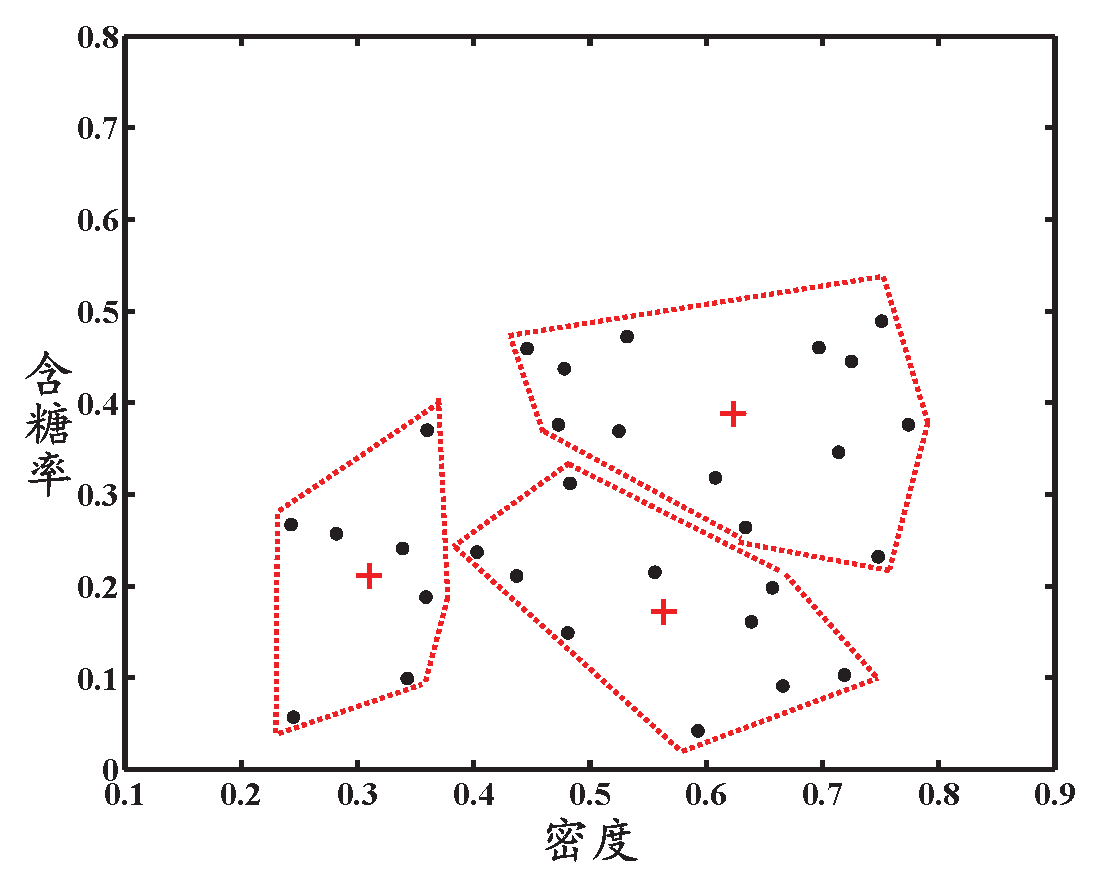
\includegraphics[width=0.45\textwidth]{pic/Fig9.3c.eps} 
	}
	\subfigure[9.3d]{
		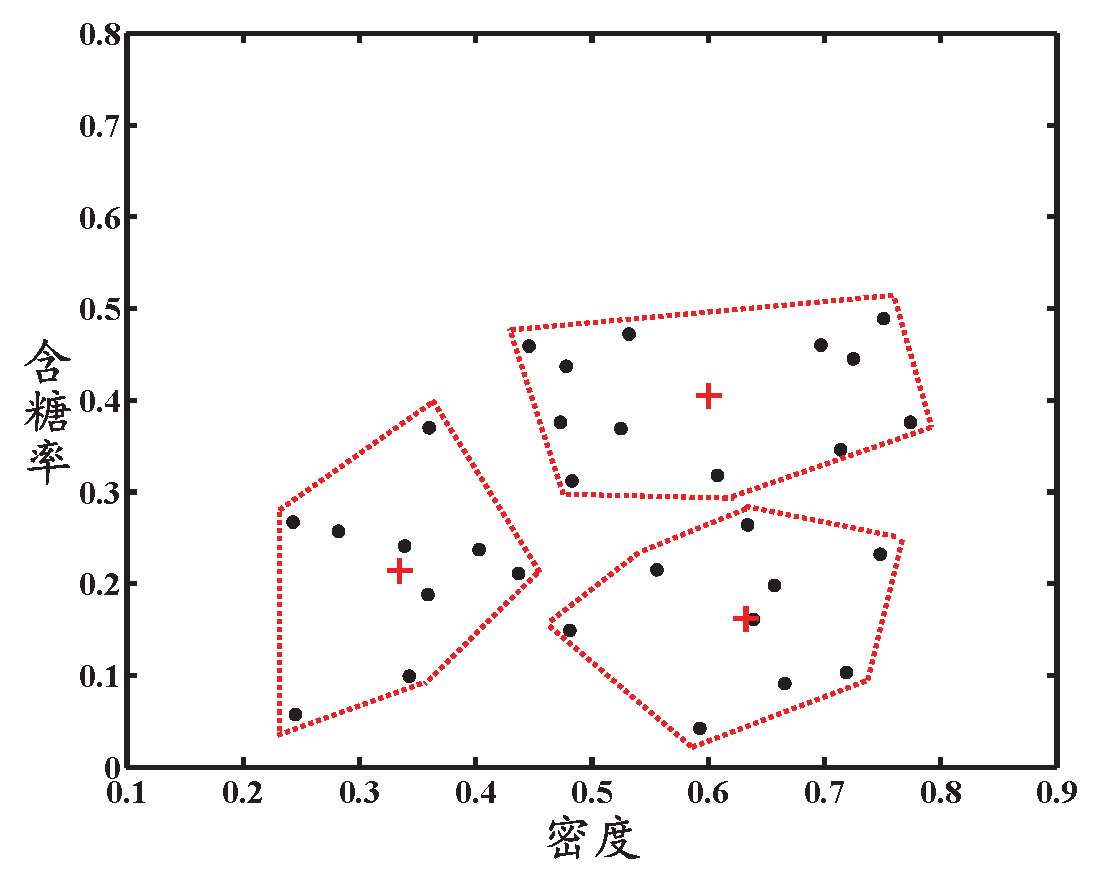
\includegraphics[width=0.45\textwidth]{pic/Fig9.3d.eps}
	}
\end{figure}\\
\\
\\
\\
\\
\\
(第一版第12次印刷, 2016年11月)
\\
(第一版第11次印刷, 2016年10月)
\\
(第一版第10次印刷, 2016年9月):
\\
p.156, 式(7.24)分母: "$N_i$" --> "$N \times N_i$" \\
p.156, 式(7.25)下面一行: "其中 $N_i$" --> "其中 $N$ 是 $D$ 中可能的类别数, $N_i$" \\
p.156, 式(7.25)下面第4行, 分母: "$17+3$" --> "$17 + 3 \times 2$" \\
p.156, 式(7.25)下面第4行: "0.350" --> "0.304" \\
\\
(第一版第9次印刷, 2016年8月)
\\
(第一版第8次印刷, 2016年5月):
\\
p.5, 第2段倒数第3行: "3、2、2" --> "3、3、3" \\
p.5, 第2段倒数第2行: "$4 \times 3 \times 3 + 1 = 37$" --> "$4 \times 4 \times 4 + 1 = 65$" \\
p.26, 边注第2行: "2.6 节" --> "2.5 节" \\
p.41, 式(2.33)上面一行: "正态分布, 且均值 …… 因此变量" --> "正态分布. McNemar检验考虑变量" \\
p.41, 式(2.33)旁加边注: "$e_{01} + e_{10}$ 通常很小, 需考虑连续性校正, 因此分子中有 $-1$ 项" \\
p.45, 第一个边注: "由式(2.37)" --> "考虑到噪声不依赖于$f$, 由式(2.37)" \\
p.63, 式(3.45)下面一行: "$N-1$个最大" --> "$d'$个最大非零" \\
p.63, 式(3.45)下面第2行: "矩阵." --> "矩阵, $d'\le N-1$."; 加边注: "最多有$N-1$个非零特征值" \\
p.63, 式(3.45)下面第3行: "$N-1$维" --> "$d'$维" \\
p.63, 式(3.45)下面第4行: "$N-1$通常远小于数据原有的属性数" --> "$d'$通常远小于数据原有的属性数$d$" \\
p.100, 图5.5, 左图最上面的 "阈值$0.5$" --> "阈值$1.5$" \\
p.100, 图5.5, 左图最右边的 "阈值$0.5$" --> "阈值$-1.5$" \\
p.100, 图5.5, 左图中间的"1  -1  -1  1" --> "1  1  -1  -1" \\
p.125, 式(6.18): "$y_s$" --> "$1/y_s$" \\
p.136, 式(6.54): 右边最后一项中的四处 "$i$" --> "$j$" \\
p.136, 式(6.54): 右边最后一项中最后的 "${\bm x}$" --> "${\bm x}_i$" \\
p.152, 第三个式子等号右端: "$0.375$" --> "$0.625$" \\
p.153, 第3行: "$0.038$" --> "$0.063$" \\
p.153, 第6行: "$0.038$" --> "$0.063$" \\
p.160, 式(7.29)下面第2行: "需多少字节来描述$D$" --> "对$D$描述得有多好";加边注: "可以从统计学习角度理解, 将两项分别视为结构风险和经验风险" \\
p.239, 式(10.39)第二行式子: 去掉上标 "$2$" \\
p.244, 第13行: "Locally" --> "Nonlinear dimensionality reduction by locally" \\
p.244, 第14行: "2316" --> "2326" \\
p.249, 式(11.2): "$i=1$" --> "$k=1$" \\
p.253, 倒数第5行: "[Boyd and Vandenberghe, 2004]" --> "[Combettes and Wajs, 2005]" \\
p.263, 倒数第4行, 插入: "Combettes, P. L. and V. R. Wajs. (2005). ``Signal recovery by proximal forward-backward splitting.'' \textit{Mutiscale Modeling \& Simulation}, 4(4):1168--1200." \\
p.277, 式(12.29): "$E(h) - \hat{E}(h)$" --> "$\left| E(h) - \hat{E}(h) \right|$" \\
p.299, 式(13.9)后第三段第2行: "关于 $D_u$" --> "涉及 $C_u$" \\
\\
(第一版第7次印刷, 2016年4月):
\\
p.42, 表2.5下面一段的第三行: "服从正态分布,其均值" --> "的均值" \\
p.42, 倒数第二行加边注: "原始检验要求$k$较大(例如$>30$),若$k$较小则倾向于认为无显著区别" \\
\\
(第一版第6次印刷, 2016年4月):
\\
p.56, 图3.1中,红色第一和第二个点的坐标互换 \\
p.114, 图5.15中, 卷积层 16@10x10 和 采样层 16@5x5 各去掉 8 个方块 \\
p.301, 式(13.12)的下一行: "$({\bm f}_l^{\rm T}\,{\bm f}_u^{\rm T})^{\rm T}$" --> "$({\bm f}_l^{\rm T}; {\bm f}_u^{\rm T})$" \\
p.372, 图16.2: 从"s=健康"到"s=溢水"的 "r=1" --> "r=-1" \\
p.376, 图16.5的边注: "第 4 行中式(16.4)的参数" --> "该参数在第4行使用" \\
p.385, 第二行: "在使用策略时并不需要$\epsilon-$贪心" --> "而不是为了最终使用" \\
p.387, 倒数第二行: "$\epsilon-$贪心策略, 而执行(第5行)的是原始策略" --> "原始策略, 而执行(第4行)的是$\epsilon-$贪心策略" \\
p.393, 第四段第一行: 去掉 "[Kuleshov and Precup, 2000]和" \\
p.395, 去掉最后一行 \\
p.396, 去掉第一行 \\
p.402, 式(A.32)加边注: "机器学习中 $\bf W$ 通常是对称矩阵" \\
\\
(第一版第5次印刷, 2016年3月):
\\
p.62, 第1行加边注: "$(\bm{\mu}_0 - \bm{\mu}_1)^{\rm T} \bm{w}$ 是标量" \\
p.78, 图4.4, 从右往左数: 第二个叶结点改为“好瓜”,第三个叶结点改为“坏瓜” \\
p.85, 图4.8, 从右往左数: 第二个叶结点改为“好瓜”,第三个叶结点改为“坏瓜” \\
p.85, 图4.8, 中间分支底层: “硬挺”--> “硬滑” \\
p.89, 图4.9, 中间分支底层: “硬挺”--> “硬滑” \\
p.103, 最后一行的式子: 求和的"$q$" --> "$l$" \\
p.399, 式(A.9): "$A_{1 \sigma n}$" --> "$A_{n \sigma n}$" \\
p.400, 第1行: "(1,4,3,2)" --> "(3,1,2)" \\
p.402, 式(A.32)最后一行的式子中: "$2{\mathbf A}$" --> "$2{\mathbf A}^{\rm T}$" \\
\\
(第一版第4次印刷, 2016年3月):
\\
p.59, 式(3.27)加边注: "考虑 $y_i \in \{0, 1\}$" \\
\\
(第一版第3次印刷, 2016年3月):
\\
p.15, 第5行: "居功" --> "厥功" \\
p.55, 最后一行: 式子括号中的逗号改为分号 \\
p.125, 第3行: "减小" --> "增大" \\
p.125, 第4行,第6行: "减幅" --> "增幅" \\
p.125, 第5行: "减小" --> "增长" \\
\\
(第一版第2次印刷, 2016年2月):
\\
p.38, 第6行: "$\epsilon^{m'}$" --> "${m \choose m'} \epsilon^{m'}$" \\
p.119, 第14行: "318--362" --> "533--536" \\
p.404, 式(B.3)最后一行的式子 --> "$\lambda g({\bm x})=0$" \\
\\
(第一版第1次印刷, 2016年1月):
\\
p.6, 图1.2: 图中两处"清脆" --> "浊响" \\
p.28, 第3段倒数第2行: "大量" --> "不少" \\
p.28, 边注: "例如 ……上百亿个参数" --> "机器学习常涉及两类参数: 一类是算法的参数, 亦称"超参数", 数目常在10以内; 另一类是模型的参数, 数目可能很多, 例如……上百亿个参数. 两者调参方式相似, 均是产生多个模型之后基于某种评估方法来进行选择; 不同之处在于前者通常是由人工设定多个参数候选值后产生模型, 后者则是通过学习来产生多个候选模型(例如神经网络在不同轮数停止训练)." \\
p.31, 倒数第3行: "Event" --> "Even" \\
p.256, 第4段: "固定住${\bf \alpha}_i$" --> "以${\bf \alpha}_i$为初值" \\
p.256, 最后一段第1行: "${\bf E}_i =$" --> "${\bf E}_i = {\bf X} - $" \\
p.385, 式(16.25)和(16.26): 两处"$r_i$" --> "$R_i$" \\
p.385, 式(16.25)下一行: "若改用……" --> "其中$R_i$表示第$i$条轨迹上自状态$x$至结束的累积奖赏. 若改用……" \\
p.386, 式(16.28)下一行: "始终为1" --> "对于$a_i=\pi(x_i)$始终为1" \\
p.386, 图16.11, 第4步: 两处 "$\pi(x)$" --> "$\pi(x_i)$" \\
p.386, 图16.11, 第6步的式子 --> "$R=\frac{1}{T-t}\left(\sum_{i=t+1}^T r_i\right) \prod_{i=t+1}^{T-1} \frac{\mathbb I(a_i=\pi(x_i))}{p_i}$" \\
p.386, 图16.11, 边注"计算修正的累积奖赏." --> "计算修正的累积奖赏. 连乘内下标大于上标的项取值为1."; 去掉边注"重要性采样系数." \\
\\
\end{document}
